\section{Battery Management System}
INTRO HERE ------
The purpose of the Battery Management System (BMS)...
INTRO HERE ------

\subsection{Design}
Quick intro --- 

\subsubsection{Propulsion Batteries}
Battery choices...

\subsubsection{Analog Frontend}
Cell calc etc...

\subsubsection{Current Sensor}
amp measure...

\subsubsection{Isolation Switch}
safety...

\subsubsection{Digital Unit (HW)}
programming...


\subsection{Implementation}
text

\subsection{Unity test}
text

\subsection{BMS Programming Quickguide}
The purpose of this section is meant to help whoever is going to work with the BMS in the future. Here you will be guided in how to use, debug and program the Digital Unit.

Firstly, you will need a few prerequisites listed below to be able to program the BMS. Since the BMS was originally build in 2013 the software to program the BMS is outdated but sometimes it is only possible to proceed and get it to work with the specified utilities. 

Tools required to program the BMS are listed here:
	\begin{itemize}
		\item AVR Studio 4 (tested with version 4.19 Build 730).
		\item Atmel Studio 6 or 7 (Both tested).
		\item JTAG-USB programmer (programmer that is included with the BMS hardware).
		\item 2 batteries (used to power the BMS).
		\item Tera Term (or any other hyperterminal).
		\item USB-A to USB mini cable (used to debug the BMS and see readouts from Tera Term).
	\end{itemize}
	
After you have acquired these tools you are ready to proceed. First of you connect the USB cable from your computer to the BMS frontend. Then you launch your chosen hyperterminal and select the COM-port which the BMS has. Afterwards you configure the hyperterminal, where the two most important settings are the buad rate and the way you receive from the BMS. Set the baud rate to 38400, 1 stop bit, 8 data bits and 0 parity bits. Then you specify the newline settings so that you receive both CR+LF else select AUTO. In Tera Term you go to Setup->Terminal->New-line to perform these changes. 
Now you can attach the two batteries to the BMS (remember to plug in both the main plug and the cell plug to the frontend), once this is done you're ready to receive data from the frontend and it should look something like this: 
\begin{figure}[H]
	\centering
	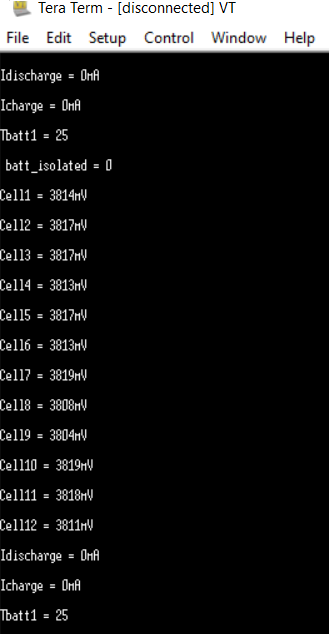
\includegraphics[width=0.6\linewidth]{Hardware/Pictures/BMS_teraterm}
	\caption{Tera Term Printout from BMS}
	\label{fig:BMSTeraTerm}
\end{figure}

Now you're ready to program the BMS. You can compile the code from either Atmel Studio 6 or 7, when you're done compiling you'll have a .hex file which is used for the AVR-CAN (Digital Unit). From this point on you have to follow the guide located in the pdf-file "How-to-install-and-use-AVR-JTAG-USB.pdf" which is located in the BMS repository. Now you can program the AVR-CAN module by selecting the .hex file or other valid files and program the BMS.

You can always confirm the programming by looking at the hyper terminal printouts and see if it matches your expectations. However, if it does not match your expectations you will have to debugg the source code or the hardware to resolve the problem.

